% Copyright (c) 2014,2016 Casper Ti. Vector
% Public domain.

\chapter{谱线对低高度小尺度加热的响应}\label{chap:5}
在这一章节中我们利用RH代码对太阳上低高度、小尺度的加热现象产生的Mg \textsc{ii}线和H$\alpha$线进行模拟。之所以不使用IRIS另外观测的C \textsc{ii}线和Si \textsc{iv}线的原因是C \textsc{ii}线存在计算时的数值崩溃或不能收敛的问题,可能来自于某些高温大气造成的原子能级粒子数在LU分解中产生奇异性。而Si \textsc{iv}线已经在\ref{sec:3.8}节中的讨论中证明不包含Si \textsc{i}和\textsc{ii}能级的Si原子文件不适合对Si \textsc{iv}谱线的形成进行模拟。因此我们把目光投向Mg \textsc{ii}线和H$\alpha$线,计算在低高度出现小尺度加热时的谱线轮廓变化。
\section{研究方法}
为了研究的方便,我们在这里仅采取一种半经验的方法,通过人工在RH的输入大气中在低高度上的几个格点的温度进行修改。整个插入过程依靠的是我自己临时编写的一个可视化ipython小程序(见~\ref{sec:a.1.3})。同时我们没有给RH代码输入电子密度随高度的分布,故其将自动根据我们的提供的温度信息迭代计算该高度上的NLTE电离下的电子密度。在得到RH代码计算的谱线之后,我们将这些谱线和紫外爆发以及Ellerman炸弹的典型光谱进行比较,希望能够寻找到拟合较好的谱线轮廓,帮助我们更好地认识这些在色球,乃至光球层次上的小尺度加热过程。
\section{初始设置}
我在宁静太阳VALC大气的五个高度点0.25, 0.5, 0.75, 1.0和1.5 Mm上分别尝试插入了一些温度比原有温度高$2\times10^3-4\times10^5$ K不等的温度,具体插入的数值可以参见表~\ref{Table2}和图~\ref{fig:5.1}。注意图~\ref{fig:5.1}中的电子密度$n_e$已经是经过RH代码计算后的结果。显然插入一个局域的温度上升能够提高局地的电子密度,而且插入的位置温度越低,相同的温度升高反而能导致更多的H \textsc{i}原子电离,产生相对更大的电子密度增加。此外值得一提的一点是为了简化操作量我并没有在响应的高度上插入速度的双向流。这对较低高度上的Ellerman炸弹的模拟可能并无太大影响,因为在光球小尺度的加热并不会产生非常大的宏观体速度流\parencites{Hong2017b}。而对于发生在较高高度的紫外爆发,它们一般会形成较大的速度流和较宽的谱线轮廓。

\begin{table}
	\centering
	\begin{tabular}{cccc}
	\hline
    高度 (Mm) & 温度1 (kK) & 温度2 (kK) & 温度3 (kK)  \\ 
 	\hline
    0.25 & 6 & 8 & 10 \\
    0.50 & 6 & 8 & 10\\
    0.75 & 6 & 10 & 20 \\
    1.00 & 8 & 15 & 20 \\
    1.50 & 10 & 20 & 50 \\
    \hline
\end{tabular}
    \caption{本实验中插入温度的数值和其插入高度}\label{Table2}
\end{table}

\begin{figure}
	\centering
	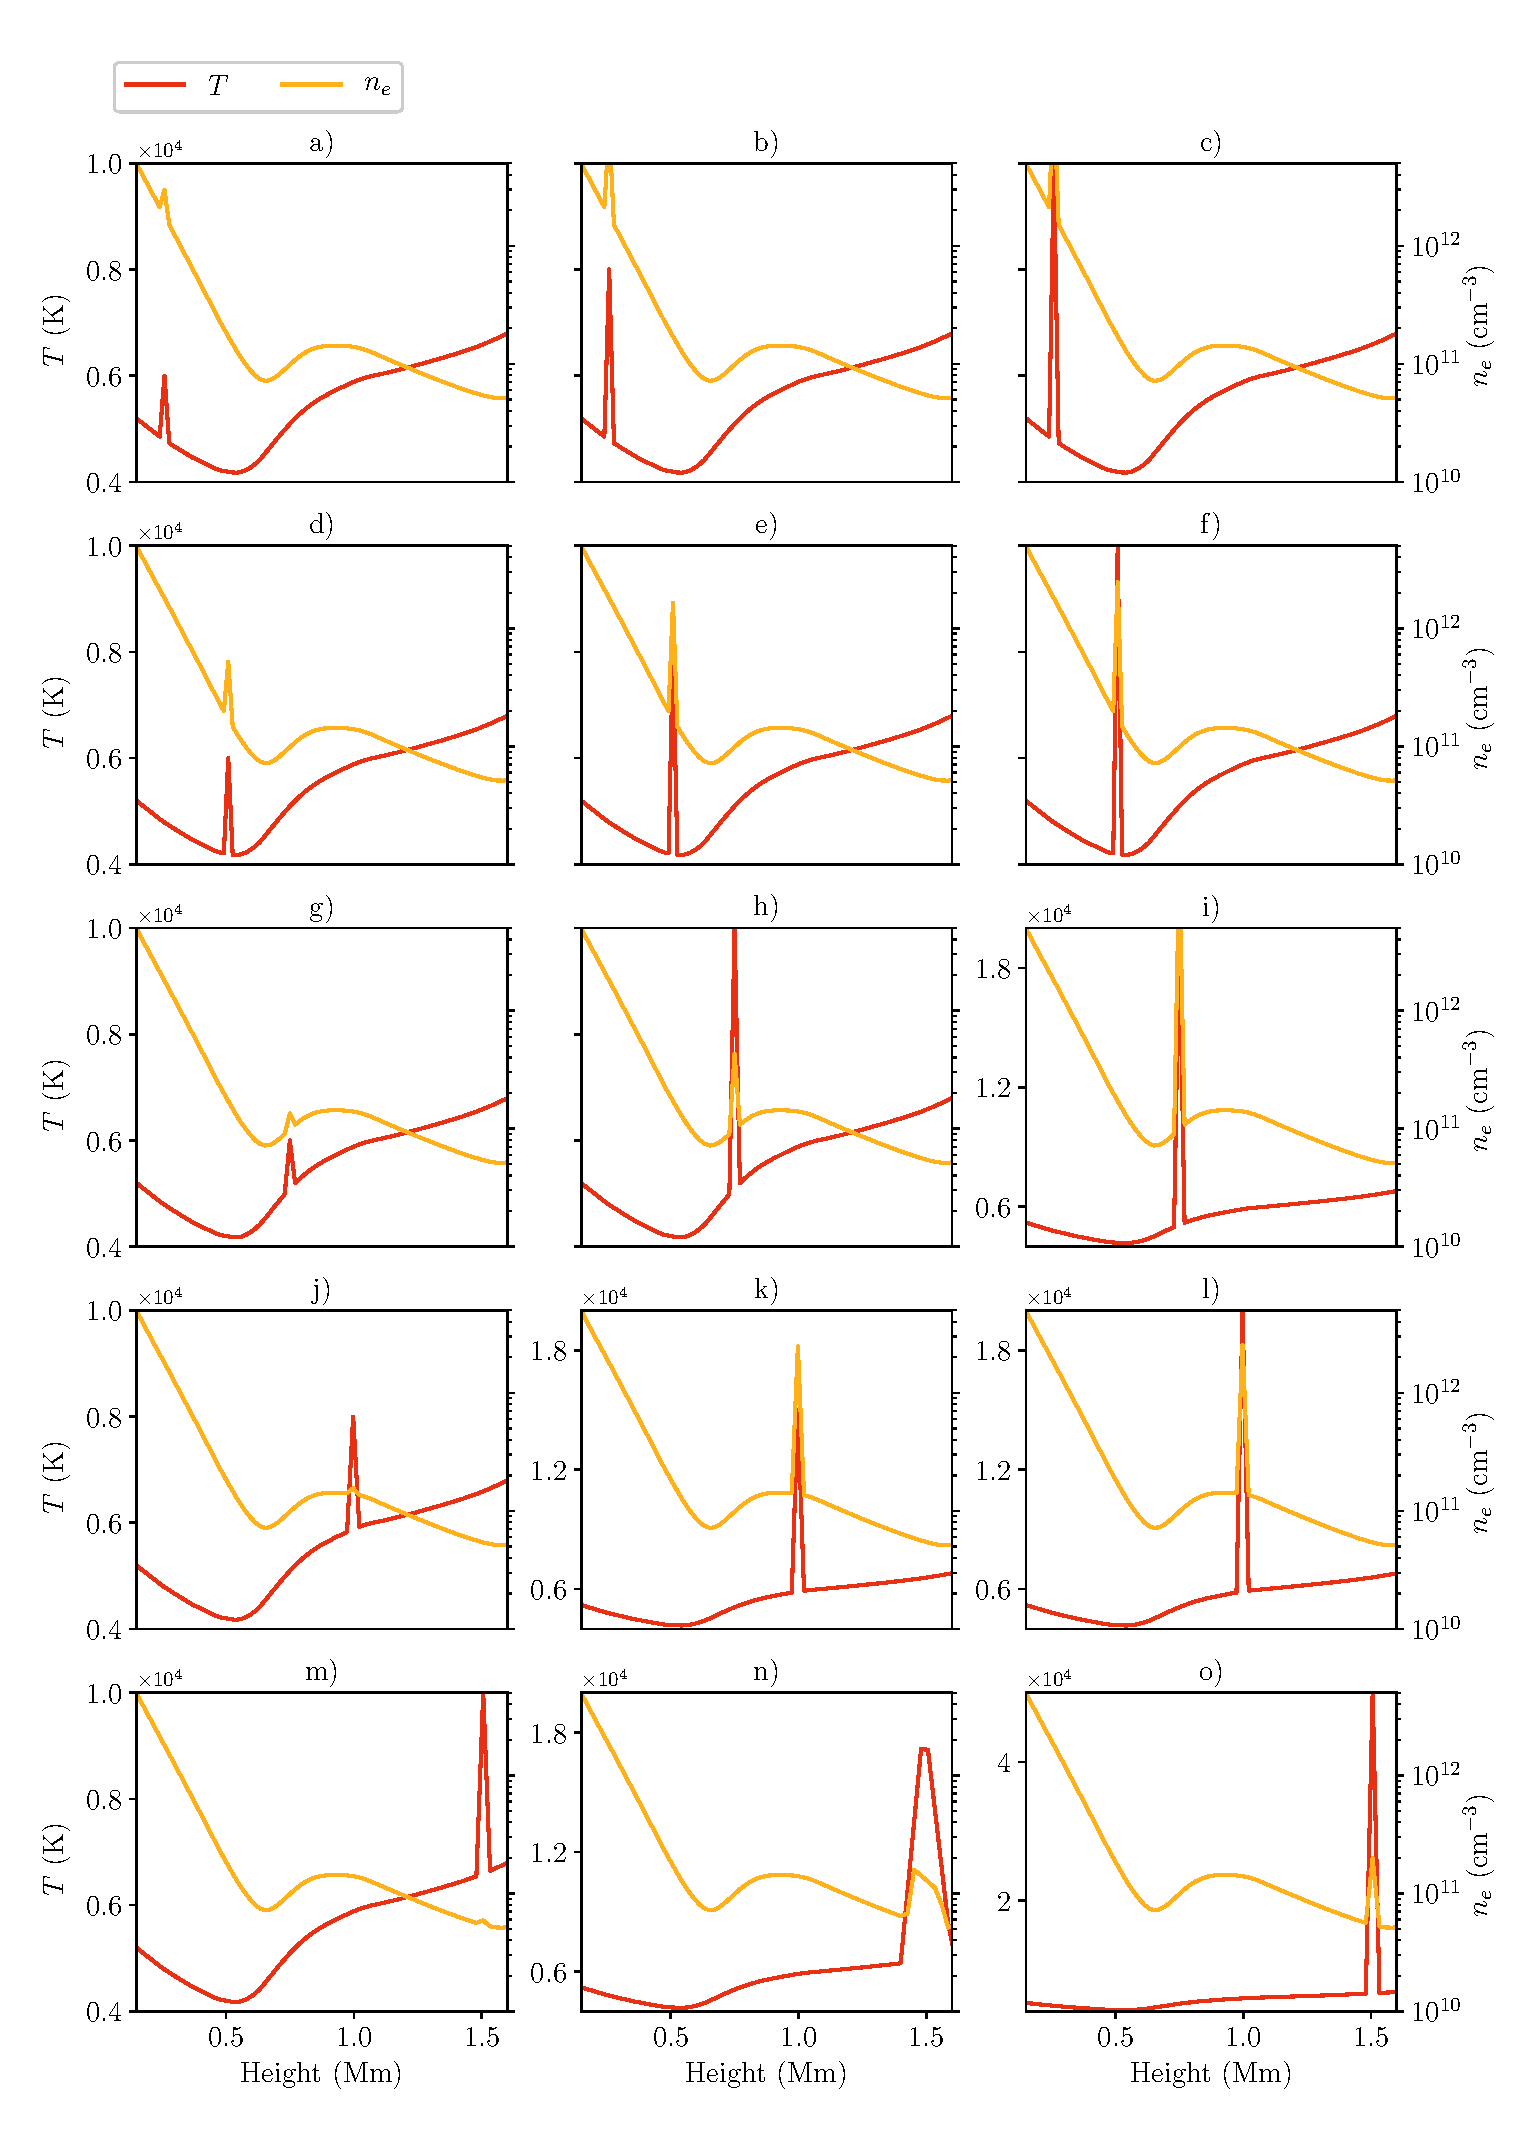
\includegraphics[width=\textwidth]{figs/UVB_atoms}
	\caption{模拟中所使用的经过手动插入温度后的大气模型中温度$T$与电子密度$n_e$随高度的分布。注意其中的电子密度已经是经过RH代码计算后的结果。}
	\label{fig:5.1}
\end{figure}
\section{合成光谱与讨论}在这一部分我们将集中展示在各个大气中计算得到的光谱和实际观测到的光谱的比较。从图~\ref{fig:5.2},\ref{fig:5.3}和\ref{fig:5.4}中可以看到,不同高度不同程度的温度增加,得到了轮廓各异的Mg \textsc{ii}线和H$\alpha$线。在这里,我们不妨对生成的这些谱线对应的大气加热模型的特点做一些归纳:
\begin{enumerate}
	\item 三条谱线都没有明显增强的有a、d、g、j和m栏。这些大气模型的特点就是温度增加不够大,因此无法对周边的原子能级占据数和谱线形成产生影响。
	\item Mg \textsc{ii} h线翼都明显增强的大气模型有c、e、i、f、h、k和l栏。它们的突出特征是在0.25 Mm和1 Mm之间有接近$10^4$ K的温度。
	\item Mg \textsc{ii} 2791 \mbox{\AA}在此时体现出其对低层大气加热的敏感性,较小程度的低层大气加热或只加热高层大气,都不会反映在在Mg \textsc{ii} 2791 \mbox{\AA}谱线轮廓变化上。其线翼增强与Mg \textsc{ii} h线翼的增强保持了比较高的一致性且与观测光谱在线心部分能够得到比较好的拟合。但在低色球加热时整个谱线轮廓并不是\textcites{Pereira2015}中所提到的出现发射线,而仍是伴随着线翼增强的吸收线。
	\item 部分在Mg \textsc{ii} h远线翼出现增强的模型,如b和c,对应着在光球高度发生的局部温度增加。在它们的H$\alpha$合成光谱中,增加温度较小(到约$\sim 8$ kK)的模型出现了$H\alpha$谱线线心和线翼位置的辐射减小,而增加到$10$ kK的模型出现了线心和线翼(主要是在线翼)的辐射增强。这和\textcites{Hong2017b}中对Ellerman炸弹进行数值模拟发现在开始阶段H$\alpha$谱线出现整个谱线轮廓内的辐射减小相类似。尽管这个效应还没有被观测证实,但说明可能存在这样的减弱再增强的过程。
	\item 部分在高色球加热的模型,如k、l出现了Mg \textsc{ii} h线心和H$\alpha$线心线翼位置的增强。这与\textcites{Hansteen2017}中部分Ellerman炸弹和紫外爆发的谱线类似。但与实际观测还存在着一定差距。
	\item 大部分模拟都很难得到和观测非常相似的Mg \textsc{ii} h谱线轮廓,这些轮廓可能来自于模拟中尚未添加的加热区域的宏观速度出流。

\end{enumerate}




\begin{figure}
	\centering
	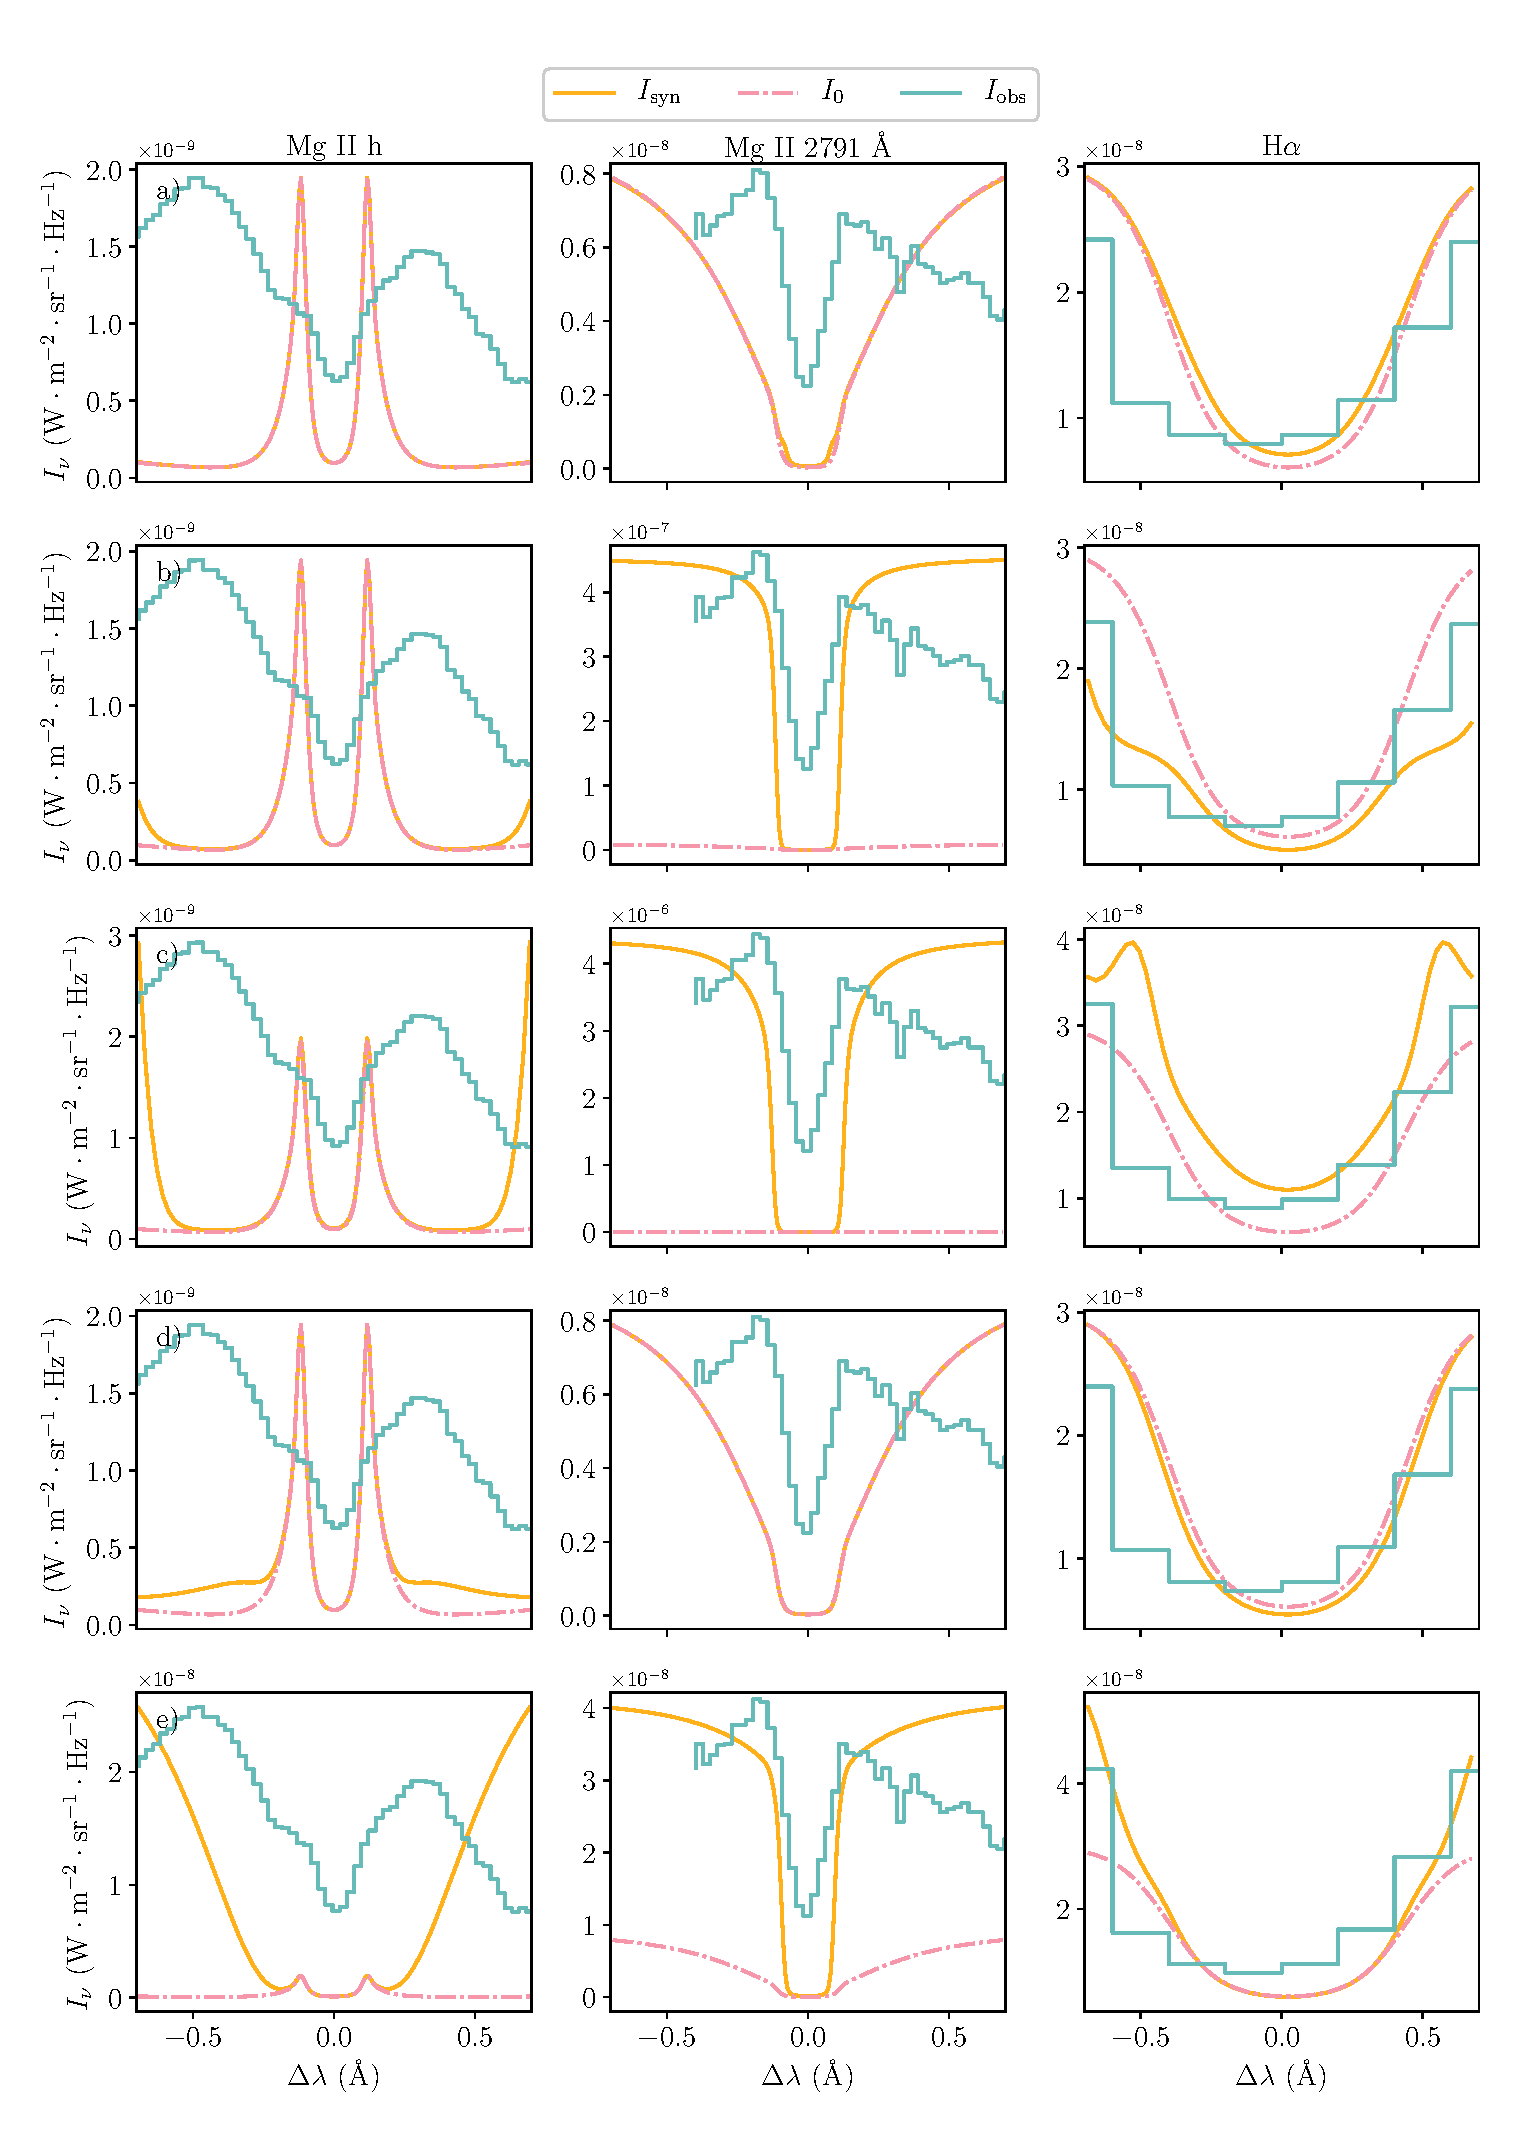
\includegraphics[width=\textwidth]{figs/UVB_spec_1}
	\caption{RH代码模拟得到的低层大气加热后的Mg \textsc{ii} h,2791 \mbox{\AA}及H$\alpha$线的谱线轮廓与IRIS卫星等观测的对比图(其一)。粉色点划线轮廓代表了初始谱线轮廓;黄色实线代表调整后计算得到的谱线轮廓。蓝色阶梯线代表实际观测的紫外爆发(Mg \textsc{ii})和Ellerman炸弹(H$\alpha$)的谱线轮廓。}
	\label{fig:5.2}
\end{figure}

\begin{figure}
	\centering
	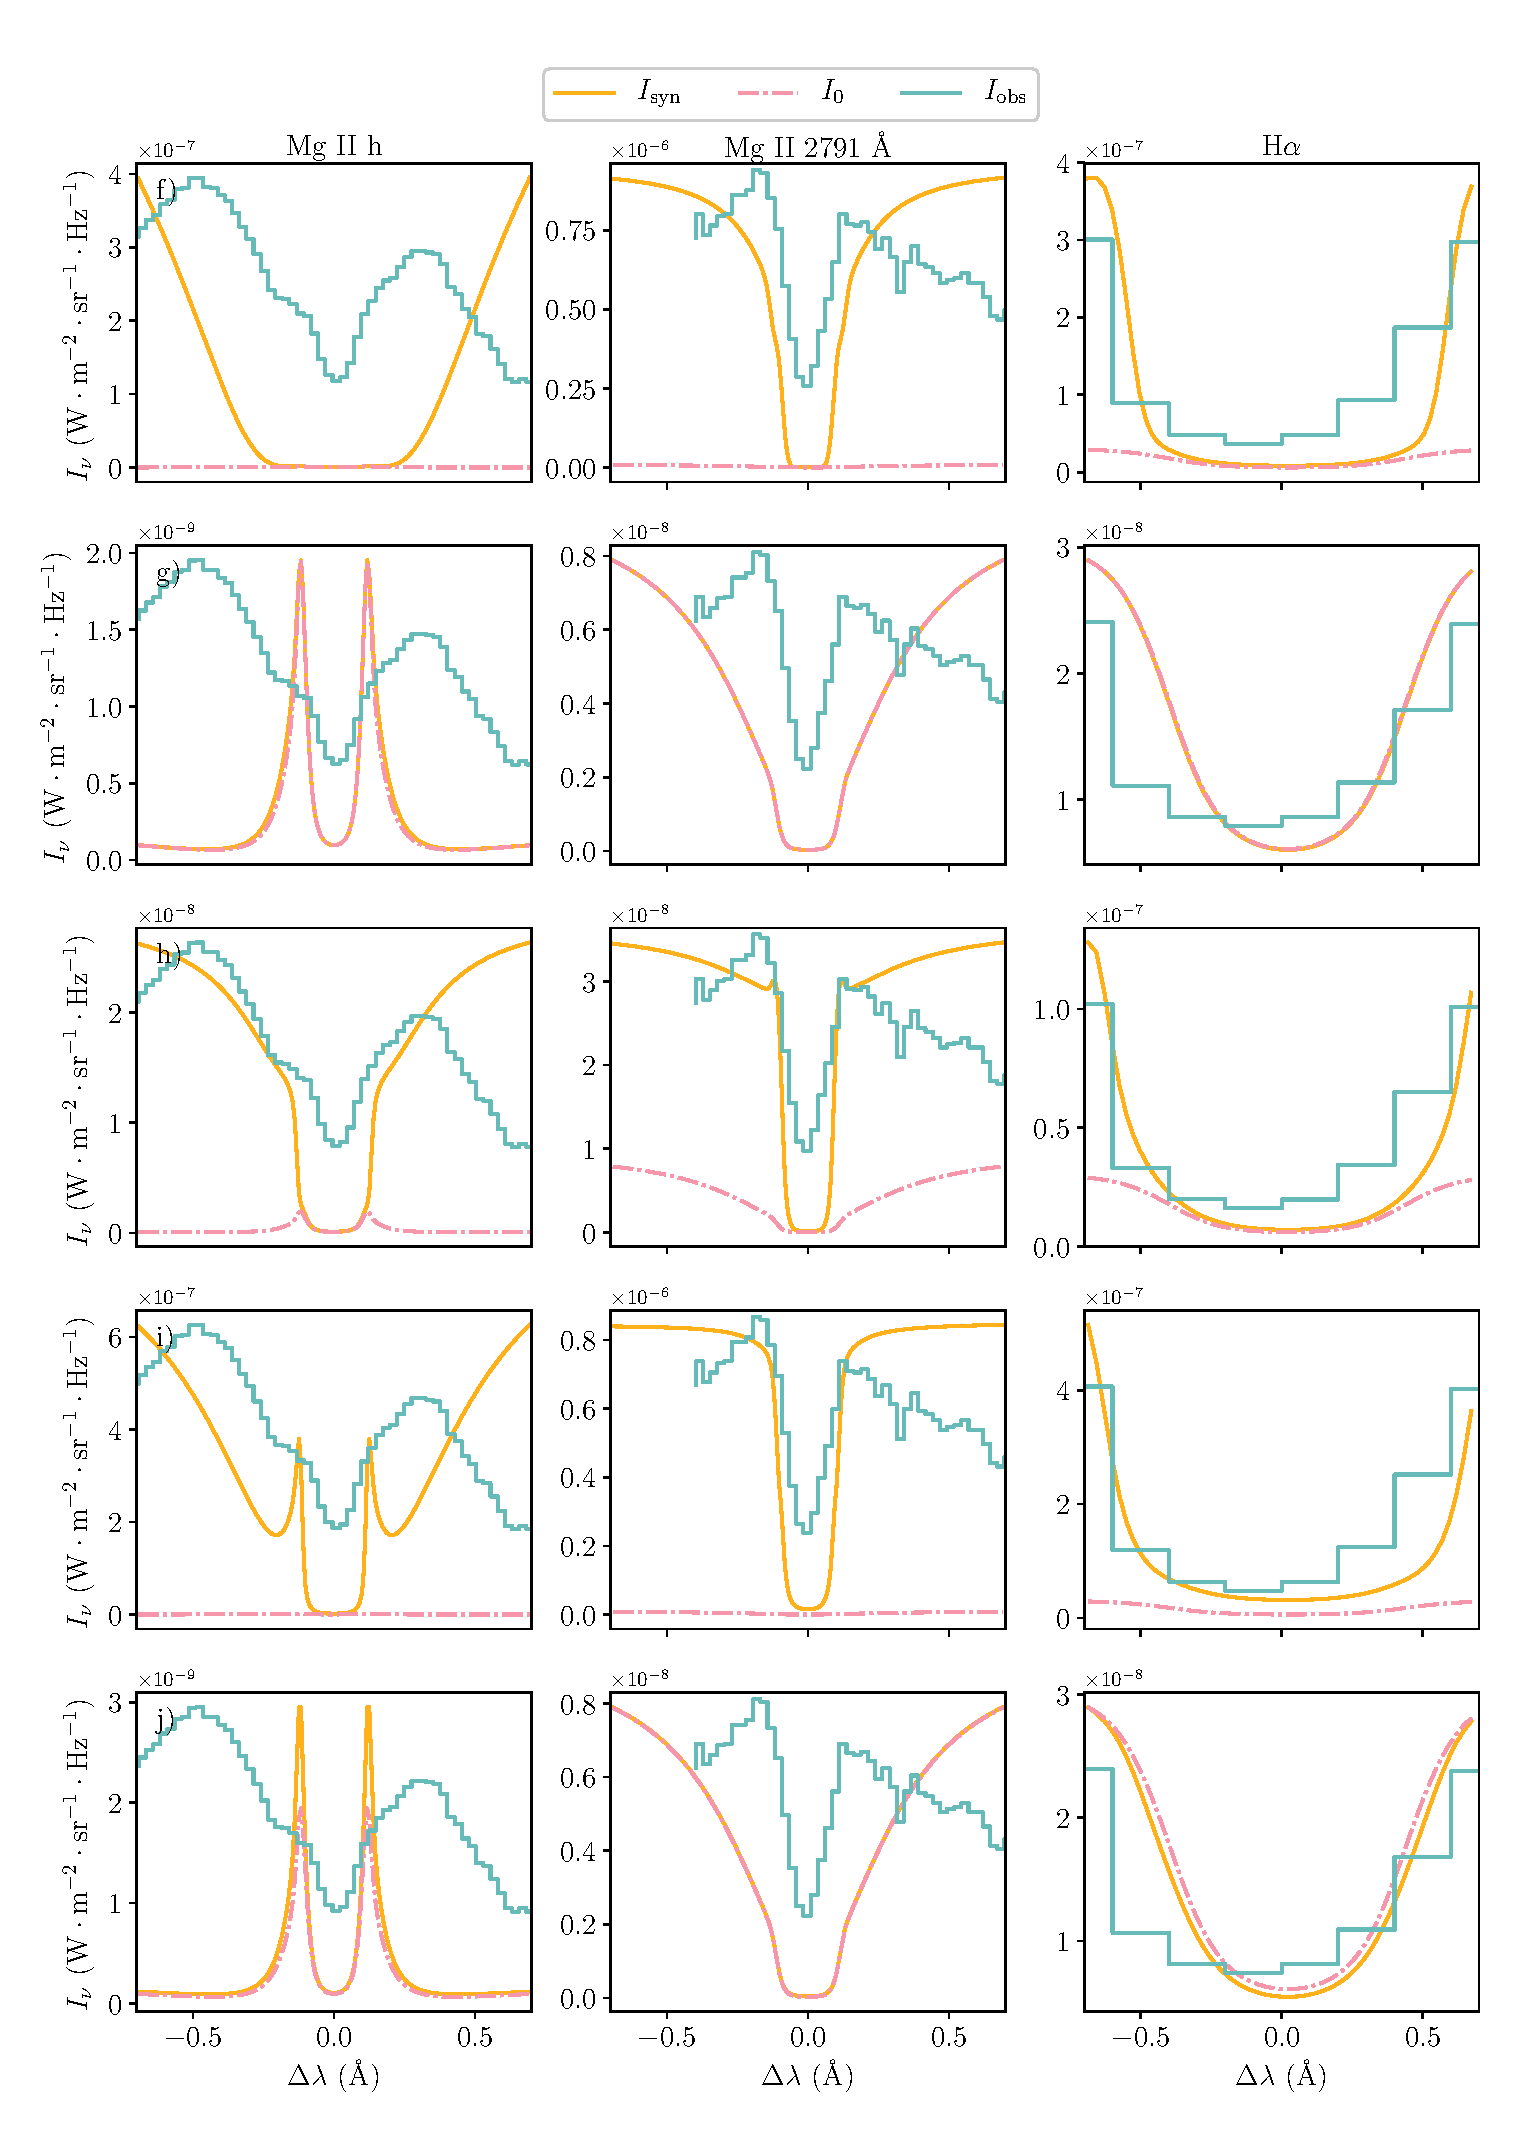
\includegraphics[width=\textwidth]{figs/UVB_spec_2}
	\caption{RH代码模拟得到的低层大气加热后的Mg \textsc{ii} h,2791 \mbox{\AA}及H$\alpha$线的谱线轮廓与IRIS卫星等观测的对比图(其二)。粉色点划线轮廓代表了初始谱线轮廓;黄色实线代表调整后计算得到的谱线轮廓。蓝色阶梯线代表实际观测的紫外爆发(Mg \textsc{ii})和Ellerman炸弹(H$\alpha$)的谱线轮廓。}
	\label{fig:5.3}
\end{figure}

\begin{figure}
	\centering
	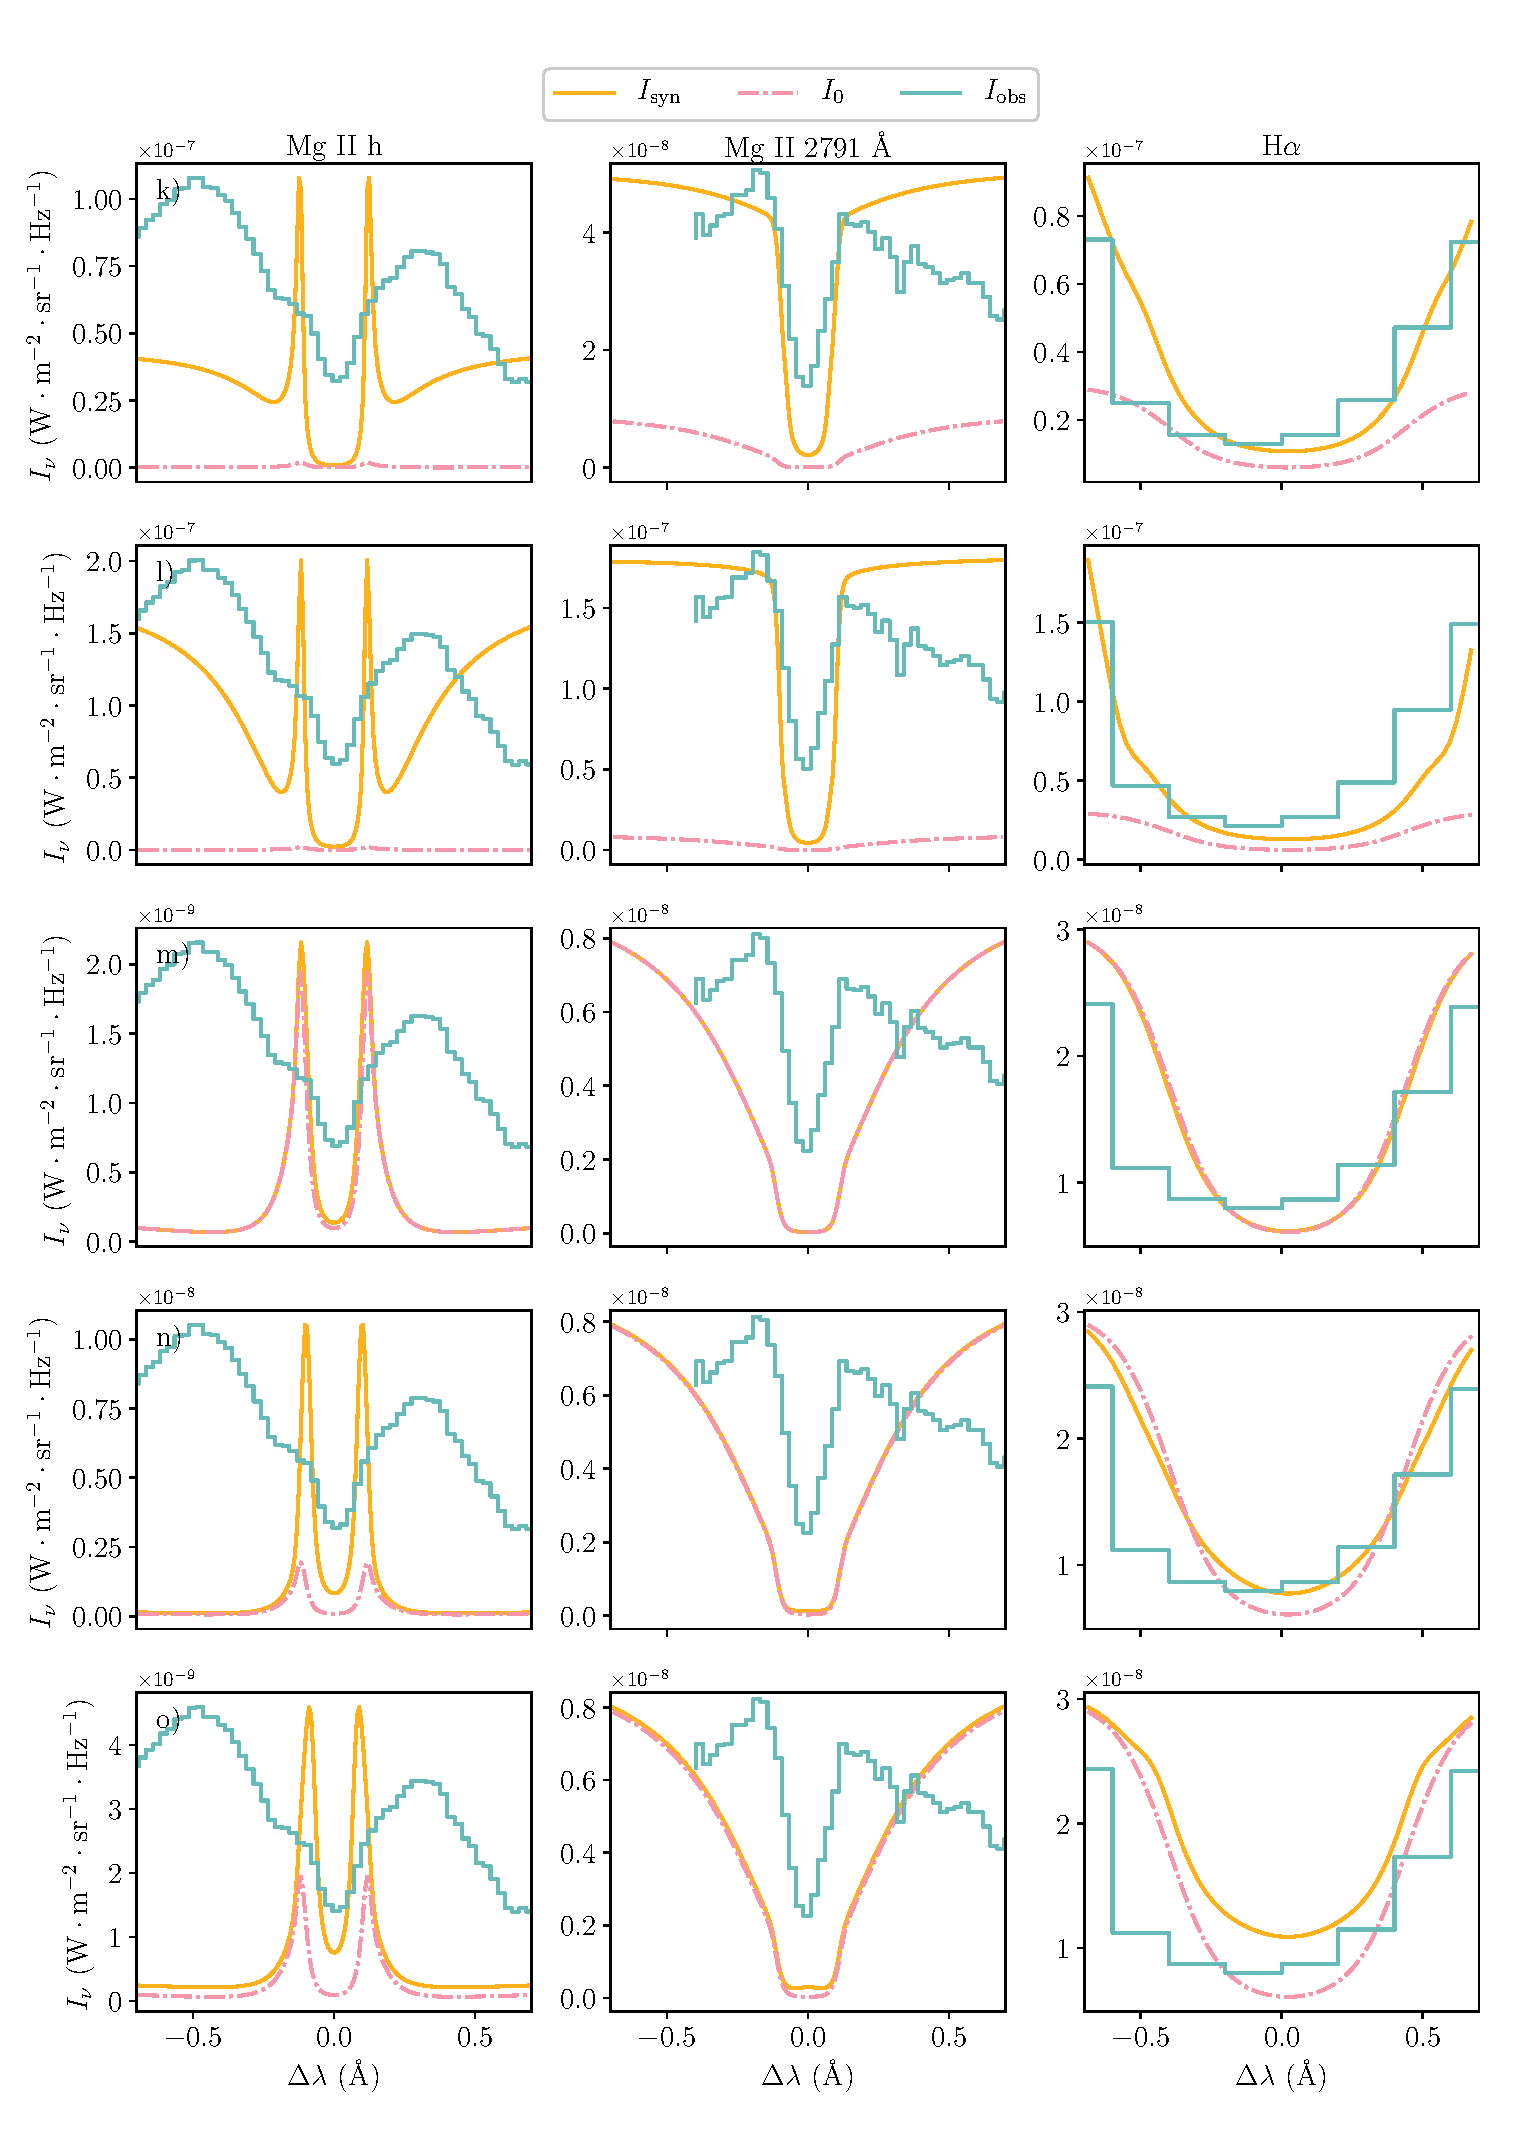
\includegraphics[width=\textwidth]{figs/UVB_spec_3}
	\caption{RH代码模拟得到的低层大气加热后的Mg \textsc{ii} h,2791 \mbox{\AA}及H$\alpha$线的谱线轮廓与IRIS卫星等观测的对比图(其三)。粉色点划线轮廓代表了初始谱线轮廓;黄色实线代表调整后计算得到的谱线轮廓。蓝色阶梯线代表实际观测的紫外爆发(Mg \textsc{ii})和Ellerman炸弹(H$\alpha$)的谱线轮廓。}
	\label{fig:5.4}
\end{figure}
% vim:ts=4:sw=4